%% ============================================================
%%  Sección 8 – Proceso AS IS: Subproceso 2
%%  Selección y Registro de Cursos
%%  Alumna responsable: Bianca Merchán Torres (20220425E)
%% ============================================================

\section{Proceso AS IS – Subproceso 2: Selección y Registro de Cursos}

El presente apartado describe el proceso actual (\emph{AS IS}) del Subproceso~2,
correspondiente a la selección y registro de cursos en la matrícula regular de la UNI.
Se expone primero el flujograma clásico del proceso y luego el modelo BPMN que
incorpora los actores y sistemas involucrados. Finalmente se ofrece una explicación
narrativa del flujo.

%% ----------------------------------------------------------
\subsection{Diagrama de Flujo}

El flujograma de la Figura~\ref{fig:asis_subproceso_2_flujo} muestra la secuencia lógica
de actividades, decisiones y flujos de retorno del Subproceso~2 en notación clásica:
óvalos para inicio/fin, rectángulos para actividades y rombos para decisiones.

\begin{figure}[H]
    \centering
    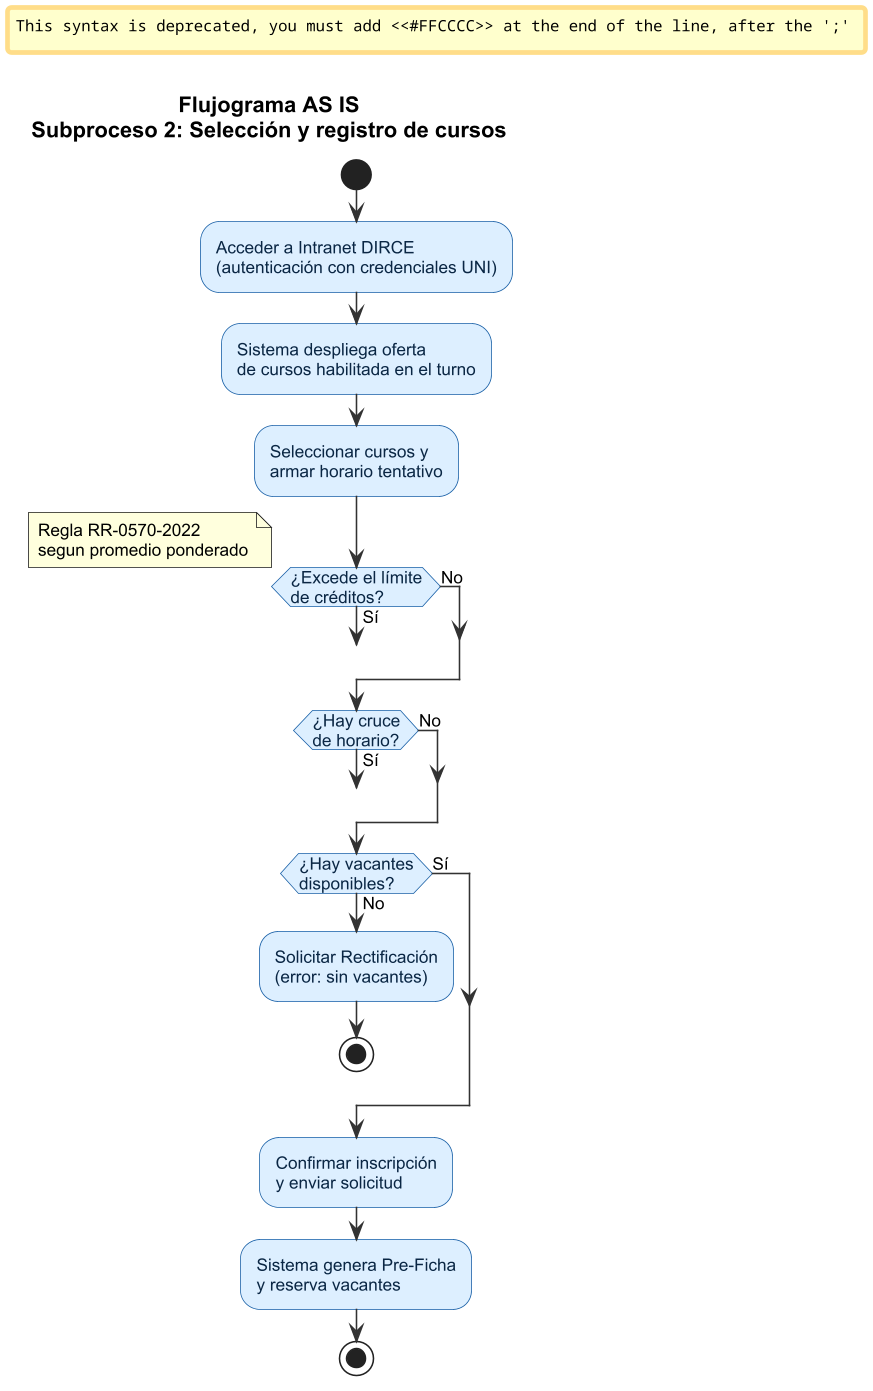
\includegraphics[width=0.72\textwidth]{asis_subproceso_2_flujo.png}
    \caption{Flujograma AS IS – Subproceso 2: Selección y Registro de Cursos.}
    \label{fig:asis_subproceso_2_flujo}
\end{figure}

El proceso inicia cuando el estudiante accede a la Intranet DIRCE con sus credenciales
institucionales. El sistema despliega la oferta de cursos habilitada para su turno de
matrícula. A continuación, el estudiante selecciona cursos y arma su horario tentativo,
enfrentando tres validaciones automáticas: (i)~límite de créditos según el promedio
ponderado acumulado (Reglamento RR-0570-2022), (ii)~cruces de horario entre cursos
seleccionados y (iii)~disponibilidad de vacantes. Las dos primeras validaciones generan
un bucle de retorno hacia la selección de cursos; la tercera, en caso de no existir
vacantes, deriva el caso al Subproceso de Rectificación (SP3A). Si todas las validaciones
son superadas, el estudiante confirma su inscripción y el sistema emite la Pre-Ficha de
matrícula reservando las vacantes correspondientes.

%% ----------------------------------------------------------
\subsection{Modelo BPMN}

El modelo BPMN de la Figura~\ref{fig:asis_subproceso_2_bpmn} representa el mismo proceso distribuido
en tres carriles (\emph{swimlanes}): Comisión de Matrícula, Sistema Intranet DIRCE /
SIGA-ORCE, y Estudiante Regular. Esta distribución permite identificar con claridad las
responsabilidades de cada actor y los puntos de interacción entre el estudiante y el
sistema institucional.

\begin{figure}[H]
    \centering
    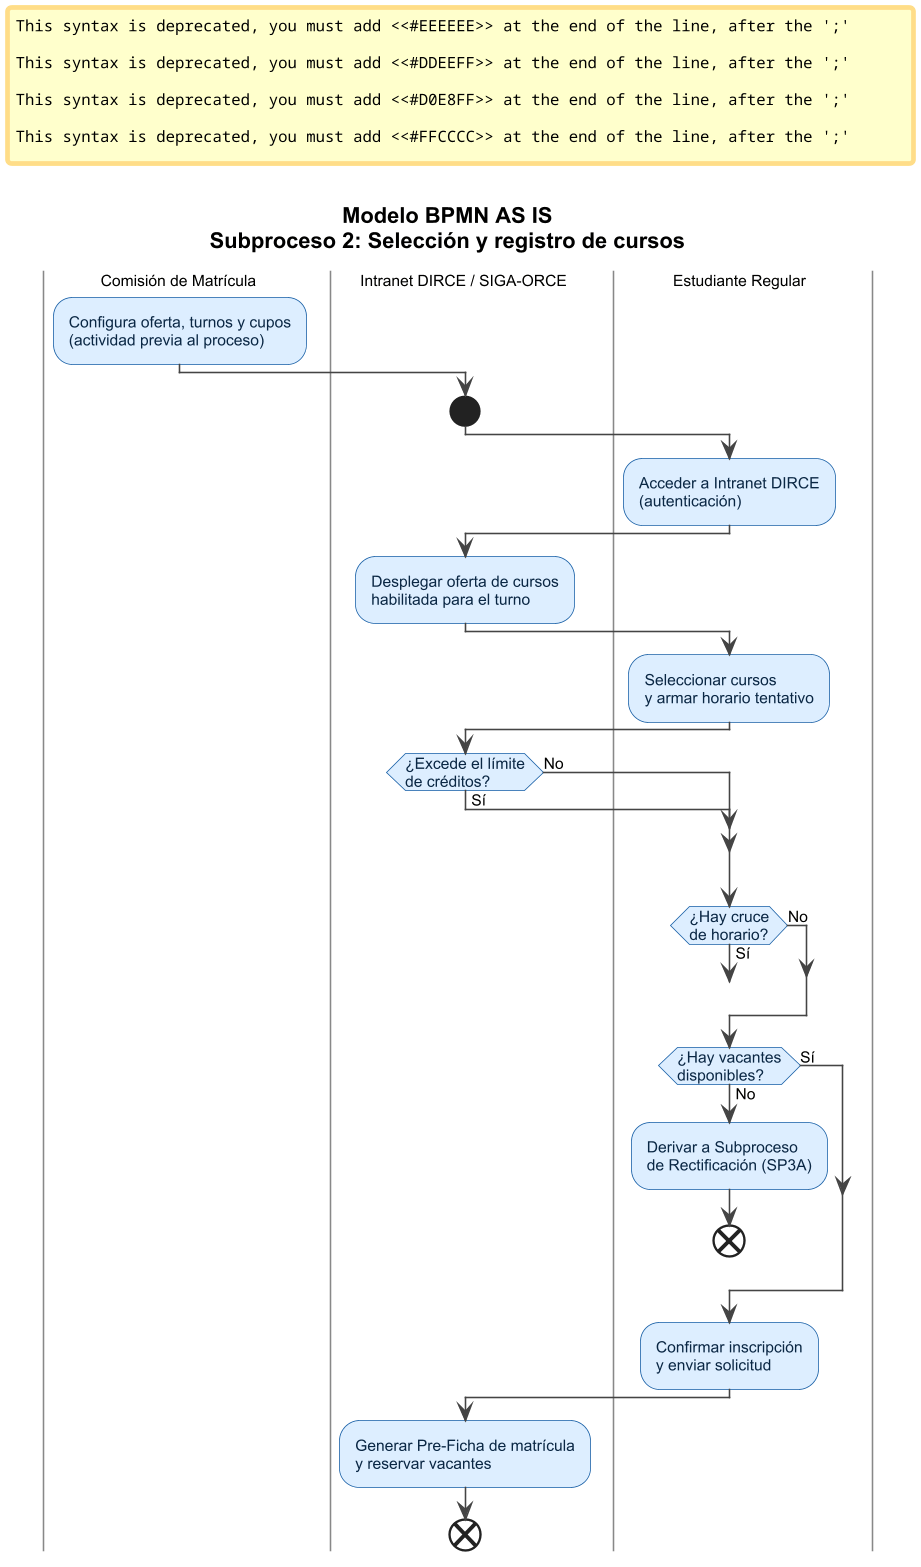
\includegraphics[width=0.95\textwidth]{asis_subproceso_2_bpmn.png}
    \caption{Modelo BPMN AS IS – Subproceso 2: Selección y Registro de Cursos.}
    \label{fig:asis_subproceso_2_bpmn}
\end{figure}

En el carril de la \textbf{Comisión de Matrícula} se configura previamente la oferta
académica, los turnos por facultad y los cupos por sección. Esta actividad precede al
inicio formal del subproceso. El carril del \textbf{Sistema (Intranet DIRCE / SIGA-ORCE)}
concentra las actividades automatizadas: autenticar al estudiante, desplegar la oferta,
ejecutar las validaciones de créditos, horarios y vacantes, y generar la Pre-Ficha de
matrícula. El carril del \textbf{Estudiante Regular} comprende las actividades
interactivas: ingresar al sistema, seleccionar y ajustar cursos, y confirmar la
inscripción.

%% ----------------------------------------------------------
\subsection{Descripción narrativa del proceso actual}

A continuación se describe el flujo paso a paso tal como ocurre en la actualidad:

\begin{enumerate}
    \item \textbf{Configuración previa (Comisión de Matrícula):} Antes de abrir el
    período de matrícula, la comisión registra en el SIGA-ORCE la oferta de cursos, los
    turnos asignados por facultad o especialidad, y los cupos máximos por sección.

    \item \textbf{Acceso al sistema (Estudiante):} El estudiante ingresa a la Intranet
    DIRCE con su código de matrícula y contraseña institucional. El sistema autentica sus
    credenciales y verifica si su turno de matrícula se encuentra vigente.

    \item \textbf{Despliegue de oferta (Sistema):} Una vez validado el turno, el sistema
    presenta la lista de cursos habilitados para el semestre, con información de horarios,
    secciones y vacantes disponibles en tiempo real.

    \item \textbf{Selección de cursos (Estudiante):} El estudiante elige los cursos de
    su plan de estudios y construye un horario tentativo. Esta actividad puede repetirse
    múltiples veces si las validaciones posteriores detectan inconsistencias.

    \item \textbf{Validación de créditos (Sistema):} El sistema calcula la suma de
    créditos de los cursos seleccionados y la compara con el límite permitido según el
    promedio ponderado acumulado del estudiante, conforme al Reglamento RR-0570-2022.
    Si el límite es superado, el estudiante debe ajustar su selección.

    \item \textbf{Validación de horarios (Sistema):} Se verifica que no existan cruces
    entre los horarios de los cursos seleccionados. Si se detecta un conflicto, el
    estudiante regresa a la etapa de selección.

    \item \textbf{Validación de vacantes (Sistema):} El sistema confirma que al menos
    una vacante esté disponible en cada sección elegida. Si no hay vacantes, el caso es
    derivado automáticamente al Subproceso de Rectificación (SP3A), donde el estudiante
    podrá solicitar un cupo adicional.

    \item \textbf{Confirmación de inscripción (Estudiante):} Superadas las tres
    validaciones, el estudiante revisa su horario final y confirma la inscripción.

    \item \textbf{Emisión de Pre-Ficha (Sistema):} El sistema registra formalmente la
    matrícula, genera la Pre-Ficha con el detalle de cursos y créditos inscritos, y
    reserva las vacantes seleccionadas para el estudiante.
\end{enumerate}

\noindent
\textbf{Problemática identificada en el proceso AS IS:} El flujo actual presenta
dependencia total de la conectividad a la Intranet DIRCE; ante caídas del sistema
durante los turnos de matrícula, el proceso queda bloqueado sin procedimiento
alternativo documentado. Asimismo, la ausencia de notificaciones proactivas obliga al
estudiante a monitorear manualmente la disponibilidad de vacantes, generando reingresos
repetidos al sistema. Estos problemas se abordan en la propuesta de mejora (proceso
TO BE) del Subproceso~2.
